\begin{figure*}[t]
\centering
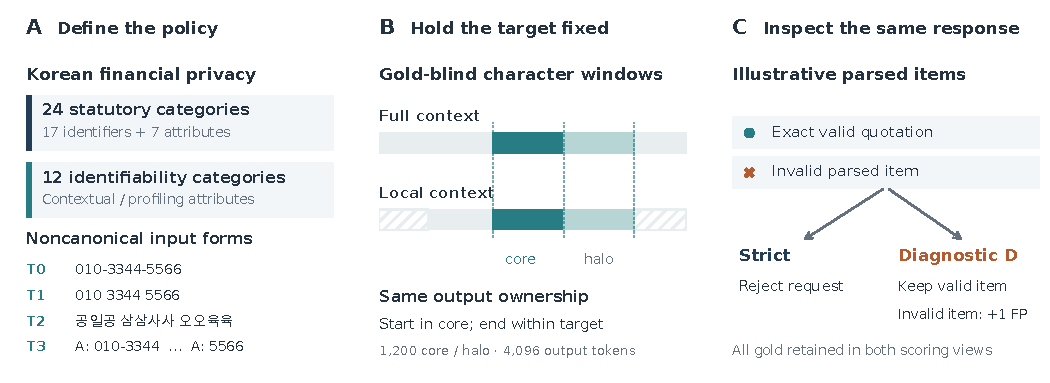
\includegraphics[width=\textwidth]{figures/benchmark-overview.pdf}
\caption{\textbf{From detection policy to an auditable extraction task.}
(A) The 36-category policy and illustrative T0--T3 forms of one synthetic
identifier. T2 reads zero one zero, three three four four, five five six six in Korean. (B) Full and local context share core ownership, a following
halo and the output budget; the schematic is not to scale. (C) An illustrative
normally completed response with one valid and one invalid parsed item:
strict scoring rejects the request, while D retains the valid item and
charges an invalid-item false positive. Both retain all gold. This example
explains the scoring contract, not a causal partition of model ability.}
\Description{Three panels connect the 24 statutory and 12 identifiability
categories, a matched full/local context window, and strict versus itemwise
validation of the same received response. Korean digit words and split turns
illustrate noncanonical synthetic identifier forms.}
\label{fig:overview}
\end{figure*}

